\documentclass[a4paper]{report}
\usepackage[utf8]{inputenc}
\usepackage[T1]{fontenc}
\usepackage[francais]{babel}
\usepackage{graphicx} 
\usepackage{fullpage}
\usepackage{hyperref}
\usepackage{xcolor}
\newcommand{\link}[1]{{\color{blue}\href{#1}{#1}}}
\usepackage{array,multirow,makecell}
\newcolumntype{R}[1]{>{\raggedleft\arraybackslash }b{#1}}
\newcolumntype{L}[1]{>{\raggedright\arraybackslash }b{#1}}
\newcolumntype{C}[1]{>{\centering\arraybackslash }b{#1}}
\newcommand{\HRule}{\rule{\linewidth}{0.5mm}}
\usepackage{eso-pic}
\begin{document}
\begin{titlepage}
\begin{center}


\includegraphics[width=0.35\textwidth]{./images/ESTS_logo.png}~\\[2cm]
{\huge \bfseries Rapport du PFE}\\[0.4cm]
% Title
\HRule \\[0.4cm]
{\huge \bfseries 
\includegraphics[width=0.25\textwidth]{./images/logo.png}~\\[0.5cm]
Autour du langage de dessin vectoriel asymptote} \\[0.4cm]
\HRule \\[1.5cm]
% Author and supervisor
\begin{minipage}{0.4\textwidth}
\begin{flushleft} \large
\emph{Réaliser par:}\\
\textsc{El Mehdi El Aine}\\
\textsc{Hamza Hamdoun}\\
\textsc{Abdrahmane El Hadere}\\
\end{flushleft}
\end{minipage}
\begin{minipage}{0.4\textwidth}
\begin{flushright} \large
\emph{Encadrer par:} \\
\textsc{Mr Hamid Maarouf}\\
\emph{Tuteur:} \\
\textsc{Lbakali Hanane}\\
\end{flushright}
\end{minipage}
\vfill
% Bottom of the page
{\large Année universitaire 2020/2021}
\end{center}
\end{titlepage}
\begin{figure}
    \centering
    
\includegraphics[width=15cm]{images/rabbi zidni ilma.PNG}
\end{figure}
\newpage
\chapter*{Dédicace}
\begin{center}
\textbf{À ALLAH avant tout\\
À mes très chers parents\\}
Aucune dédicace ne saurait exprimer l’amour, l’estime, le dévouement et\\ le respect que j’ai pour vous.\\
Rien au monde ne vaut les efforts fournis jour et nuit pour mon\\
éducation et mon bien être.\\
Ce travail est le fruit de tes sacrifices que vous avez fait pour mon éducation\\et ma formation. « Je vous aime très fort »\\
\bigskip
\textbf{À mes chers frères et ma chère soeur\\}
Pour tout ce que vous avez fait pour moi ,\\Vous étiez toujours à mes côtés pour me soutenir et me motiver,\\ Je vous souhaite une vie pleine de bonheur et de succès.\\
\bigskip
\textbf{À mes chers tantes, oncles et toute ma grande famille\\}
Pour votre gentillesse, votre soutien, vos encouragements et votre\\
confiance en moi.\\
\bigskip
\textbf{À mes chers amis\\}
Pour votre gentillesse, votre compréhension, pour les beaux moments\\ qu’on a passé ensemble, ...bref pour votre amitié.\\
À mon trinôme Hamza et Abderahmane.\\
À toute personne qui m’est chère.\\
À tous ceux qui m’aiment.\\
À tous les musulmans\\
\bigskip \bigskip
\textbf{Un grand Merci à vous.}
\end{center}
\bigskip \bigskip
\begin{flushright}
\textbf{EL MEHDI EL AINE}
\end{flushright}
\addcontentsline{toc}{chapter}{Dédicace}  
\chapter*{Remerciements}
Au terme de ce travail, nous tenons à exprimer notre profonde gratitude et nos sincères remerciements pour tous ceux qui nous ont aidés de près ou de loin pendant la durée de réalisation de notre projet.\\\\
\par Nous tenons également à remercier Monsieur Hamid Maarouf, professeur à l’EST Safi pour son encadrement, son enthousiasme vis-à-vis notre projet et ses encouragements. Nos sincères remerciements sont à adresser à Mme.Lbakali Hanane qui elle a fait l’honneur de nous encadrer tout au long de ce travail. Nous l'en sommes très reconnaissants pour ses fructueux conseils et précieuses directives, et pour le grand souci qu’elle porte à l’égard de notre sujet.Un très grand merci à M.Belkharchi Driss notre ancien professeur du math au lycée 6 novembre qui nous a très aider pour la réalisation de ce projet.\\\\
\par Remerciements spéciaux à tout le corps professoral de l'EST SAfi, pour la formation de qualité qu’ils nous ont prodiguée durant ces deux années. Que tous ceux et celles qui ont contribué de près ou de loin à l’accomplissement de ce travail trouvent l’expression de nos
remerciements les plus chaleureux.
\addcontentsline{toc}{chapter}{Remerciements} 
\tableofcontents
\newpage
\listoffigures
\newpage
\listoftables
\chapter*{Introduction}
Dans ce rapport du projet de fin d'études sont présentées les différentes étapes de conception et de réalisation d’une application de bureau autour du langage de dessin vectoriel Asymptote EasyGio réaliser par le trinôme El Aine El Mehdi, Hamdoun Hamza et El Hadere Abdrahmane,en tant qu’étudiants en Génie Informatique à l’école supérieure de technologie à SAFI. L'objet principal de notre application est d'aider les élèves du lycée et leur enseignant à illustrer les notions de géométrie, et pour savoir les besoins des professeurs au niveau de géométrie on a contacté notre ancien prof, monsieur Belkharchi Driss qui nous a donné les principales parties étudier au lycée.\\
Ce rapport détaillera les différents phases dont nous sommes passées par afin d'aboutir à une application fiable et satisfaisante. Pour cela le rapport définit le travail qui nous avons effectué. Il est composée par trois grands parties. La premier partie aura pour présenter le contexte du projet et spécification des besoins, la deuxième est consacré aux conception. La dernier partie comporte les résultats obtenus.\\[0.4cm]
    \begin{figure}[!h] 
        \centering       
        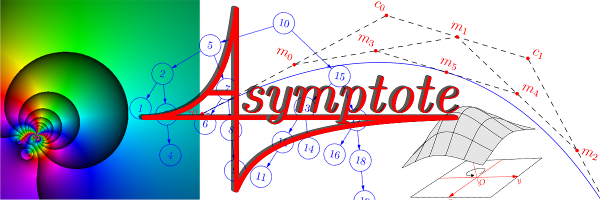
\includegraphics[width=15cm]{images/asymptote.png}\\ \caption{Asymptote} \label{Asymptote} 
    \end{figure}
\addcontentsline{toc}{chapter}{Introduction}    
\chapter{Contexte du projet}
\section{Géométrie}
\begin{figure}[!h]
    \centering
    
\includegraphics{images/fond-maths.png}
    \caption{Géométrie}
    \label{fig:Géométrie}
\end{figure}
Droites, rectangle, angles droits, polygones, axiomes, autant de termes qui appartiennent à un champ bien spécifique de l'enseignement, que tout le monde a connu ou connaîtra dans sa scolarité, voire au delà. Eh oui, la géométrie, si elle ne se résume pas à un triangle rectangle, est un champ de connaissance riche et vaste, inhérent aux maths.
Étape indispensable lors des cours traditionnels de mathématiques, la géométrie a, de tout temps, souffert d'une réputation de matière difficile! Des droits parallèles que l'on n'arrive pas à tracer, en passant par une intersection difficile à déterminer, ou des cercles peu assurés, la géométrie est parfois repoussée par les élèves.\\
Pourtant, la géométrie est particulièrement utile dans la vie de tous les jours et permet d'accéder à des carrières prestigieuses comme ingénieur ou chercheur en mathématiques. Autant de professions qui, si elles ne semblent pas être directement liées au quadrilatère et à la demi-droite, le sont bien plus qu'on ne le pense !\\
\begin{center}
La géométrie n'est pas faite pour être apprise, elle est faite pour être utilisée - Seymour Papert
\end{center}
\section{Asymptote}
    \begin{figure}[!h] \centering
        
\includegraphics[width=5cm]{images/asylogo.png}\\
        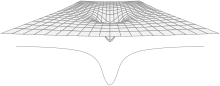
\includegraphics[width=5cm]{images/asyfonction.png}
        \caption{Asymptote} \label{Asymptote} 
    \end{figure}
\subsection{Définition}
Asymptote est un langage de description de graphismes vectoriels, particulièrement adapté pour le dessin technique. Par opposition à un logiciel classique de dessin vectoriel, il s'agit d'un langage de programmation, comme MetaPost. Asymptote possède une syntaxe proche de celle de C++, interagit naturellement avec LaTeX, étend les chemins de Metapost à la troisième dimension et gère les nombres flottants. On peut donc le considérer comme un successeur de MetaPost, mais avec une syntaxe beaucoup plus propre.
\subsection{Caractéristiques d'Asymptote}
Un avantage majeur de Asymptote sur les autres logiciels graphiques est qu'il est un langage de programmation, par opposition à juste un programme graphique. Ce qui lui donne des propriétés prenant par exemple qu'il: 
\begin{itemize}
\item Fournit un standard portable pour la composition de figures mathématiques, tout comme\\  TeX / LaTeX est devenu la norme pour la composition d'équations.
\item Génère des graphiques vectoriels PostScript, PDF, SVG, WebGL et PRC de haute qualité.
\item Incorpore des graphiques WebGL vectoriels 3D dans des fichiers HTML incorpore des graphiques   3D vectoriels PRC dans des fichiers PDF.
\item Fonctionne sur toutes les principales plates-formes (LUNIX, MacOS, Microsoft Windows).
\item Les commandes graphiques de haut niveau sont implémentées dans le langage asymptote lui-même, ce qui leur permet d'être adaptées à des applications spécifiques.
\end{itemize}
\newpage
\subsection{Les fonctions}
Asymptote est le seul langage que nous connaissons de cela
traite les fonctions comme des variables, mais autorise la surcharge
en distinguant les variables en fonction de leurs signatures.\\
En fait, les définitions de fonctions ne sont que du "syntactic sugar -en anglais-", conçu pour rendre les choses plus faciles à lire ou à exprimer. Cela rend le langage «plus doux» pour l'usage humain, les choses peuvent être exprimées de manière plus claire, plus concise ou dans un style alternatif que certains préfèrent, pour affecter des objets de fonction à des variables:\smallskip\\
\textbf{real square(real x) return $x^2$;}\\
est équivalant à\\
\textbf{real square(real x);  square=new real(real x) return $x^2$;}\smallskip\\
 \par Asymptote prend en charge un mécanisme plus flexible pour les arguments de fonction par défaut que C++: ils peuvent apparaissent n'importe où dans le prototype de fonction. Cette fonctionnalité sous-tend la plus grande force d'Asymptote, des valeurs par défaut raisonnables pour les éléments graphiques de base permettent de créer de superbes graphiques et dessins avec des scripts extrêmement courts, sans sacrifier le flexibilité pour une personnalisation détaillée. Les arguments par défaut sont évalués comme des expressions Asymptote dans le portée où la fonction est définie.\\
Paramètres du reste permettent d'écrire des fonctions prendre un nombre variable d'arguments. Par exemple, la fonction suivante additionne ses arguments:\\
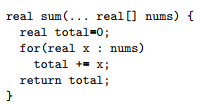
\includegraphics[width=5cm]{images/cap2.png}\\
\par Comme dans d'autres langues modernes, les fonctions peuvent appeler
eux-mêmes récursivement. Opérateurs, y compris tous les
Les opérations d'arithmétique et de chemin intégrées d'Asymptote,
ne sont que du syntactic sugar pour des fonctions qui peuvent être
adressé et défini avec le mot-clé opérateur.
Les fonctions asymptotes sont des valeurs de première classe, ce qui leur permet d'être définies dans, transmises à et
renvoyé par d'autres fonctions. Ceci est pratique lorsque
on veut tracer une séquence de fonctions telles que:
\textbf{fn(x) = n sin($x/n$) for  n = 1 to 5 from x = −10 to 10}\\
    \begin{figure}[!h] 
        \centering
        
\includegraphics[width=5cm]{images/cap1.png}
        \caption{Fonction arithmétique} 
        \label{Fonction arithmétique}
    \end{figure}
\newpage
\subsection{Les modules}
Asymptote est actuellement livré avec des dizaines des modules de base qui étend les capacités mathématiques d'Asymptote avec des fonctions utiles.
\subsubsection{Markers}
Le module Markers fournit tout ce qu’il faut pour marquer segments et angles, il permet, entre autres, de marquer d’un trait (ou deux, ou. . .) des segments de droites.
Prenant par exemples les marqueurs des segments suivant:\\
{\color {blue} StickIntervalMarker}\\\\

\includegraphics{images/Des1.png}\\
Code:\\
\textbf{import markers;\\
size(7cm,0);\\
pair A=(0,0), B=(3,0);\\
draw(A--B,StickIntervalMarker(2,2,bp+green,dotframe(red)));\\
label("\$A\$",A,W);label("\$B\$",B,E);}\\\\
{\color{blue} CrossIntervalMarker}\\\\

\includegraphics{images/Des2.png}\\
Code:\\
\textbf{import markers;\\
size(7cm,0);\\
pair A=(0,0), B=(3,0);\\
draw(A--B,CrossIntervalMarker(2,4,bp+green,dotframe(red)));\\
label("\$A\$",A,W);label("\$B\$",B,E);}\\\\
{\color{blue} CircleBarIntervalMarker}\\\\

\includegraphics[]{images/Des3.png}\\
Code:\\
\textbf{import markers;\\
size(7cm,0);\\
pair A=(0,0), B=(3,0);\\
draw(A--B,CircleBarIntervalMarker(2,0,radius=1.2mm,bp+green,\\ filltype=NoFill,dotframe(red)));\\
label("\$A\$",A,W);label("\$B\$",B,E);}\\\\
{\color{blue} TildeIntervalMarker}\\\\

\includegraphics{images/Des4.png}\\
Code:\\
\textbf{import markers;\\
size(7cm,0);\\
pair A=(0,0), B=(3,0);\\
draw(A--B,TildeIntervalMarker(2,1,size=1mm,bp+green,above=false,\\
dotframe(red)));\\
label("\$A\$",A,W);label("\$B\$",B,E);}\\\\
\subsubsection{Graph}
\begin{center}
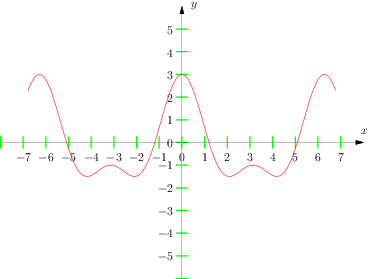
\includegraphics[width=10cm]{images/Des5.png}\\
\end{center}
Code:\\
\textbf{import graph;\\
unitsize(8mm);\\
xaxis(Label("\$x\$",position=EndPoint,align=NE),xmin=-8,xmax=8,\\
ticks=Ticks(endlabel=false,beginlabel=false,Step=1,end=false,\\
pTick=bp+green),Arrow);\\
yaxis(Label("\$y\$",position=EndPoint,align=NE),ymin=-6,ymax=6,\\
ticks=Ticks(endlabel=false,beginlabel=false,Step=1,end=false,\\
pTick=bp+green),Arrow);\\
real f(real x) {return 2cos(x) + cos(2x);}\\
path p=graph(f,-2*pi-.5,2*pi+.5,operator ..);\\
draw(p,red);}\\
\subsubsection{Three}
Le module three apporte un grand nombre d’outils permettant de faciliter la construction des figures 3D ,ce module permet de construire les sphères,les cubes..etc\\
Prenant par exemple le code suivant qui nous donne un sphère:\\
Code:\\
\textbf{import three;\\
size(2.5cm, 0);\\
draw(unitsphere,\\
surfacepen=material(diffusepen=red,\\
emissivepen=black specularpen=black));}\\
\begin{center}
    
\includegraphics{images/Des6.png}
\end{center}
\newpage
\section{Cadre de projet}
\subsection{Objectifs du projet}
Ce projet vise principalement à améliorer un service qui aide les élèves du lycée et leurs enseignant à illustrer les notions de géométrie. L’objectif de ce projet est de déployer une application Windows qui se caractérise par une haute disponibilité ,une simplicité et la multiplication des choix.Par conséquence cela revient à déployer une application EasyGio qui répond aux exigences suivants:
\begin{itemize}
    \item Faciliter l'utilisation de l'application EasyGio pour le client.
    \item Éviter les tâches répétitives et faciliter la personnalisation EasyGio.
    \item Inclure des multiples fonctions pour la conceptions des différents figures.
    \item Conception d'une interface graphique simple et facile à utiliser.\\
\end{itemize}
\begin{figure}[!h]
    \centering
    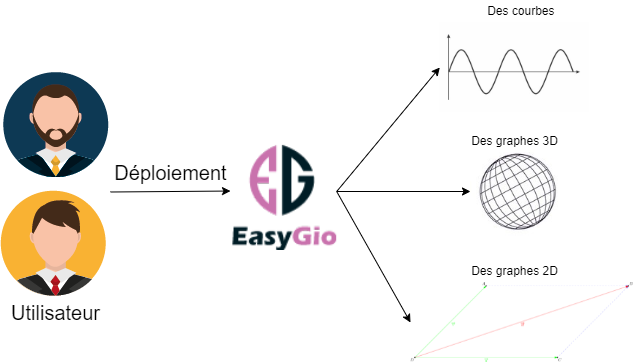
\includegraphics[width=13cm]{images/EasyGioServices.png}
    \caption{Processus souhaité de déploiement des services EasyGio}
    \label{fig:Processus souhaité de déploiement des services EasyGio}
\end{figure}
\subsection{Planification du projet}
Notre projet est loin d’être classique. En effet, il fait appel aux technologies non abordées le long de notre parcours scolaire. Du coup, une planification rigoureuse s’est imposée pour prévoir le déroulement du projet. Grâce aux réunions tenues avec notre encadrante , nous avons été éclairés sur les différentes étapes du projet ainsi que leurs séquencements. Le projet est partagé en trois grandes étapes : la première est une phase de documentation dont les objectifs est de bien assimiler les nouveaux concepts concernant les langages de programmation Asymptote et Python, d’autre part de délimiter le périmètre du projet au niveau
fonctionnel qu’au niveau technique. La seconde partie est consacrée à la conception de la solution, quant à la troisième étape, elle traite la mise en œuvre de la solution à travers la réalisation, les tests, et le déploiement.\\
Le projet a débuté le 1 mars pour une durée de 3 mois. Il en résulte le planning suivant :
\begin{figure}[!h]
    \centering
    \rotatebox{-90}{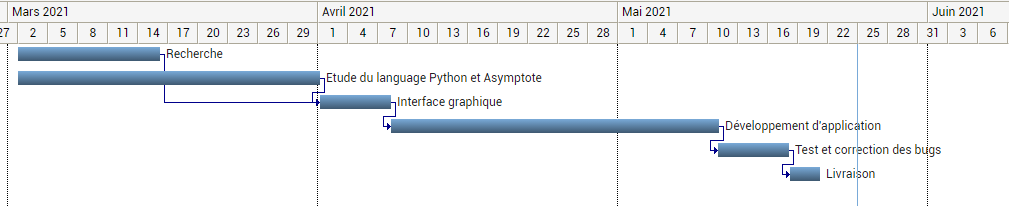
\includegraphics[width=23cm]{images/Ganter.png}}
    \caption{Diagramme de Gantt}
    \label{fig:Diagramme de Gantt}
\end{figure}
\chapter{Conception et réalisation}
\section{Diagramme des cas d'utilisations}
\begin{figure}[!h]
    \centering
    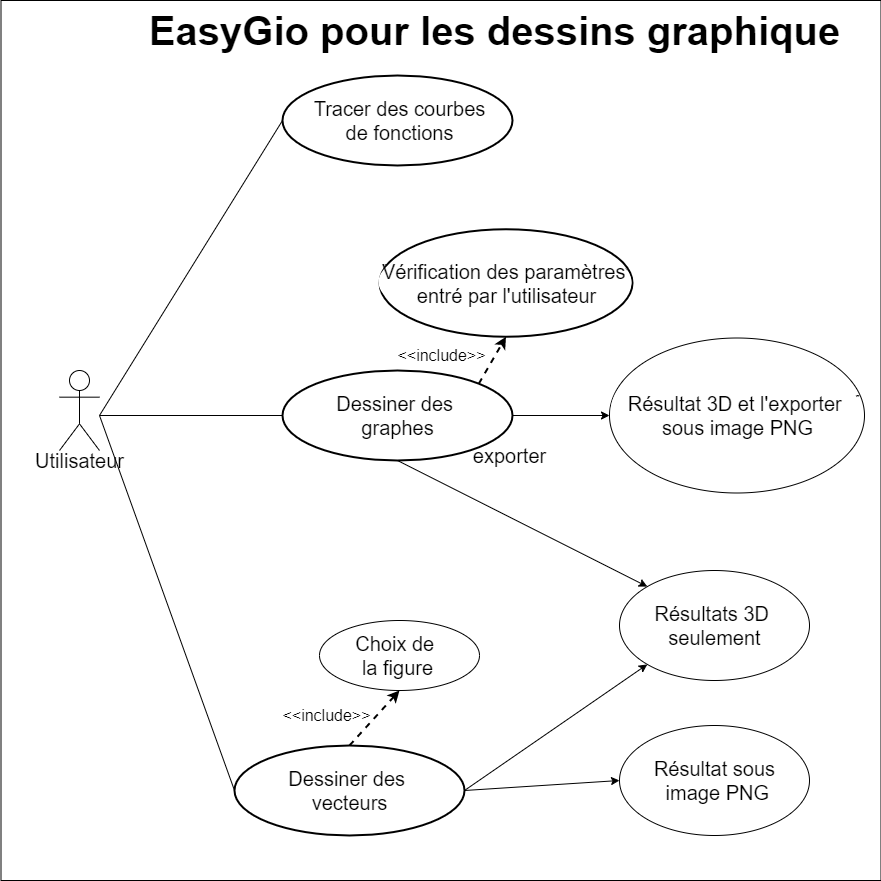
\includegraphics[width=14cm]{images/MY UML.PNG}
    \caption{Cas d'utilisation normale pour l'application}
    \label{fig:Cas d'utilisation normale pour l'application}
\end{figure}
\newpage
\begin{table}[!h]
    \centering
    \begin{tabular}{|L{5cm}|L{10cm}|}
        \hline
        \multirow{3}{4em}{\textbf{Titre :}}&\\& Diagramme de cas d'utilisation normale.\\&\\
        \hline
        \multirow{3}{4em}{\textbf{Acteur :}}&\\&Utilisateur , Système. \\&\\
        \hline
        \multirow{3}{4em}{\textbf{Raffinement du diagramme : }}&\\&  Aucun.\\&\\
        \hline
        \multirow{5}{4em}{\textbf{Précondition :}} 
        &\\& Installation de Python3.\\& Installation d'une distribution latex.\\& Installation d'Asymptote sous latex.\\&\\
        \hline
        \multirow{8}{4em}{\textbf{Description :}}
         &\\& L'utilisateur peut construire des diffèrent graphe des fonction définit avec seul variable x, et in-définit avec deux variable x et y.\\& L'utilisateur peut construire des graphe 3D avec des tailles différents.\\& L'utilisateur peut construire des graphe sur les vecteur 2D sous image PNG.\\& L'utilisateur peut construire des graphe 3D et le transformer sous image PNG.\\& L'utilisateur peut retourner vers la dernière page en appuyant sur la bouton Retourner.\\& L'utilisateur peut retourner vers la page d'accueil en appuyant sur la bouton Annuler.\\&\\
        \hline
         \multirow{3}{4em}{\textbf{CasDérivé :}} &\\& Si Python ou latex ou Asymptote ne sont pas installé correctement l'application ne peut pas être lancer. \\&\\
        \hline
        \multirow{3}{4em}{\textbf{PostCondition :}}&\\& Interface affichées. \\&\\
        \hline
    \end{tabular}
    \caption{Détails du diagramme des cas d'utilisations pour l'application}
    \label{tab: Détails du diagramme des cas d'utilisations pour l'application}
\end{table}
\section{Diagramme de séquence}
Le diagramme de séquence représente la succession chronologique des opérations réalisées par un acteur.Il indique les objets que l'acteur va manipuler et les opérations qui font passer d'un objet à l'autre.\\
Puisque notre application n'utilise ou  ne traître pas des informations saisi par l'utilisateur alors on n'utilise pas une base de données pour gérer les données de l'application, Alors il y'aura une interaction entre l'utilisateur et l'application.
\begin{figure}[!h]
    \centering
    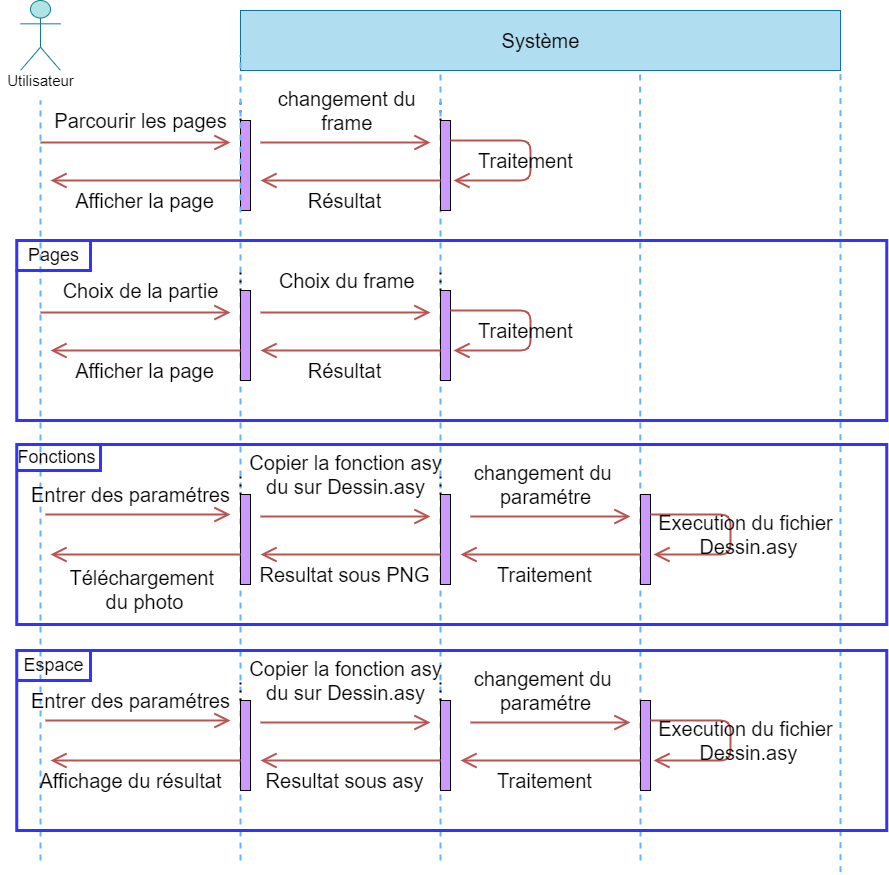
\includegraphics[width=11cm]{images/DS.png}
    \caption{Diagramme de séquence}
    \label{fig:Diagramme de séquence}
\end{figure}
\newpage
\section{Work Breakdown Structure}
Une structure de répartition du travail (WBS) est une dé-construction visuelle, hiérarchique et orientée livrable d'un projet. C'est un diagramme utile pour les chefs de projet car il leur permet de travailler à rebours à partir du livrable final d'un projet et d'identifier toutes les activités nécessaires pour réussir un projet.
\begin{figure}[!h]
    \centering
    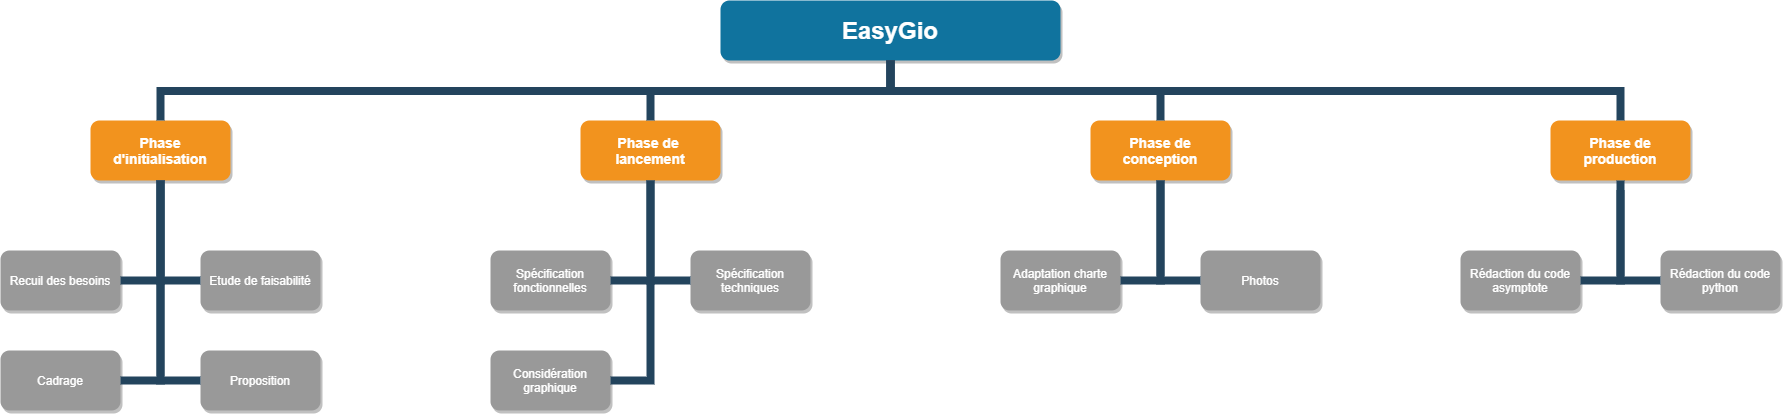
\includegraphics[width=15cm]{images/WBS.png}
    \caption{WBS diagram}
    \label{WBS diagram}
\end{figure}
\newpage
\section{Environnements de travail et choix techniques}
Cette section met l’accent sur les logiciels utilisés durant ce travail. Puis nous abordons les choix des différentes technologies mises en place.
\subsection{Environnements de travail}
Les principaux logiciels utilisé durant la conception d'EasyGio sont:
\begin{itemize}
    \item \textbf{Visual studio code :} Afin d’avoir une bonne aide au développement ainsi qu’une bonne intégration des dfférents outils python Visual Studio Code fut utilisé tout au long du développement, c'est un éditeur de code extensible ses fonctionnalités incluent la prise en charge du débogage, la mise en évidence de la syntaxe, la complétion intelligente du code, les snippets, la refactorisation du code et Git intégré et des extensions qui ajoutent des  fonctionnalités supplémentaires.
    \item  \textbf{Miktex :} C'est une distribution TeX libre pour Windows visant à fournir un environnement TeX/LaTeX complet et prêt à utiliser, pour exécuter les fichier asymptote et rédiger le rapport.
    \item  \textbf{Microsoft Office :} World 2019 pour la rédaction du cahier des charges.
    \item  \textbf{Gantter project :} Pour la rédaction du diagramme gant.
    \item  \textbf{Adobe :} utilisé pour le traitement des images utilisées tout le long du projet que ce soit dans la conception du logo dans le rapport élaboration du cahier de charge ou le développement de l’application.
    \item  \textbf{Draw.io:} Pour la rédaction des différents diagrammeS et organigrammes pour le rapport.
\end{itemize}
\subsection{Langage de programmation et technologies utilisés}
Durant notre travail, on a utiliser plusieurs outils et technologies :
\subsubsection{Asymptote}
Asymptote est le Langage de programmation utilisé pour les dessins géométrique pour notre \\application 
\subsubsection{Git}
Pour la gestion de version, étant habitué à Git. Cet outil nous a permis tout au long du PFE de garder trace des différentes évolutions de celui-ci. L’un des avantage de Git est sa gestion aisée des branches. Cette fonctionnalité est très utile pour tester sans crainte certaines approches et d’en garder une trace même si en l’état ces modifications ne sont prêtes pour rejoindre le tronc commun.
\subsubsection{Python}
Python est un langage de programmation interprété, orienté objet et de haut niveau avec une sémantique dynamique. Ses structures de données intégrées de haut niveau, associées à un typage dynamique et à une liaison dynamique, le rendent très attractif pour le développement rapide d'applications, ainsi que pour une utilisation d'interface graphique on utilisant la bibliothèque Tkinter le meilleur choix pour une application graphique simple rapide et facile à utiliser.\newpage
\subsection{Les bibliothèques Python utilisé}
\subsubsection{Tkinter}
Tkinter (" Tk Inter face") est le package multi-plateforme standard de python pour la création d'interfaces utilisateur graphiques (GUI). Il donne accès à un interpréteur Tcl sous-jacent avec la boîte à outils Tk, qui est elle-même une bibliothèque d'interface utilisateur graphique multiplateforme et multilingue.
Tkinter n'est pas la seule bibliothèque graphique pour python, mais c'est celle qui est fournie en standard. Les bibliothèques GUI supplémentaires pouvant être utilisées avec python incluent wxPython , PyQt et kivy .\\
La plus grande force de Tkinter réside dans son omniprésence et sa simplicité. Il fonctionne directement sur la plupart des plates-formes (Linux, OSX, Windows) et comprend un large éventail de widgets nécessaires pour les tâches les plus courantes (boutons, libellés, dessin, texte
multiligne, etc.).\\
On a utilisé la bibliothèque Tkinter pour la conception d'interface graphique de notre application EasyGio  en ajoutant des multiple pages , texte et des boutons pour se naviguer entre ces frames et la réception du commande par le client ou l'utilisateur. 
\begin{figure}[!h]
    \centering
    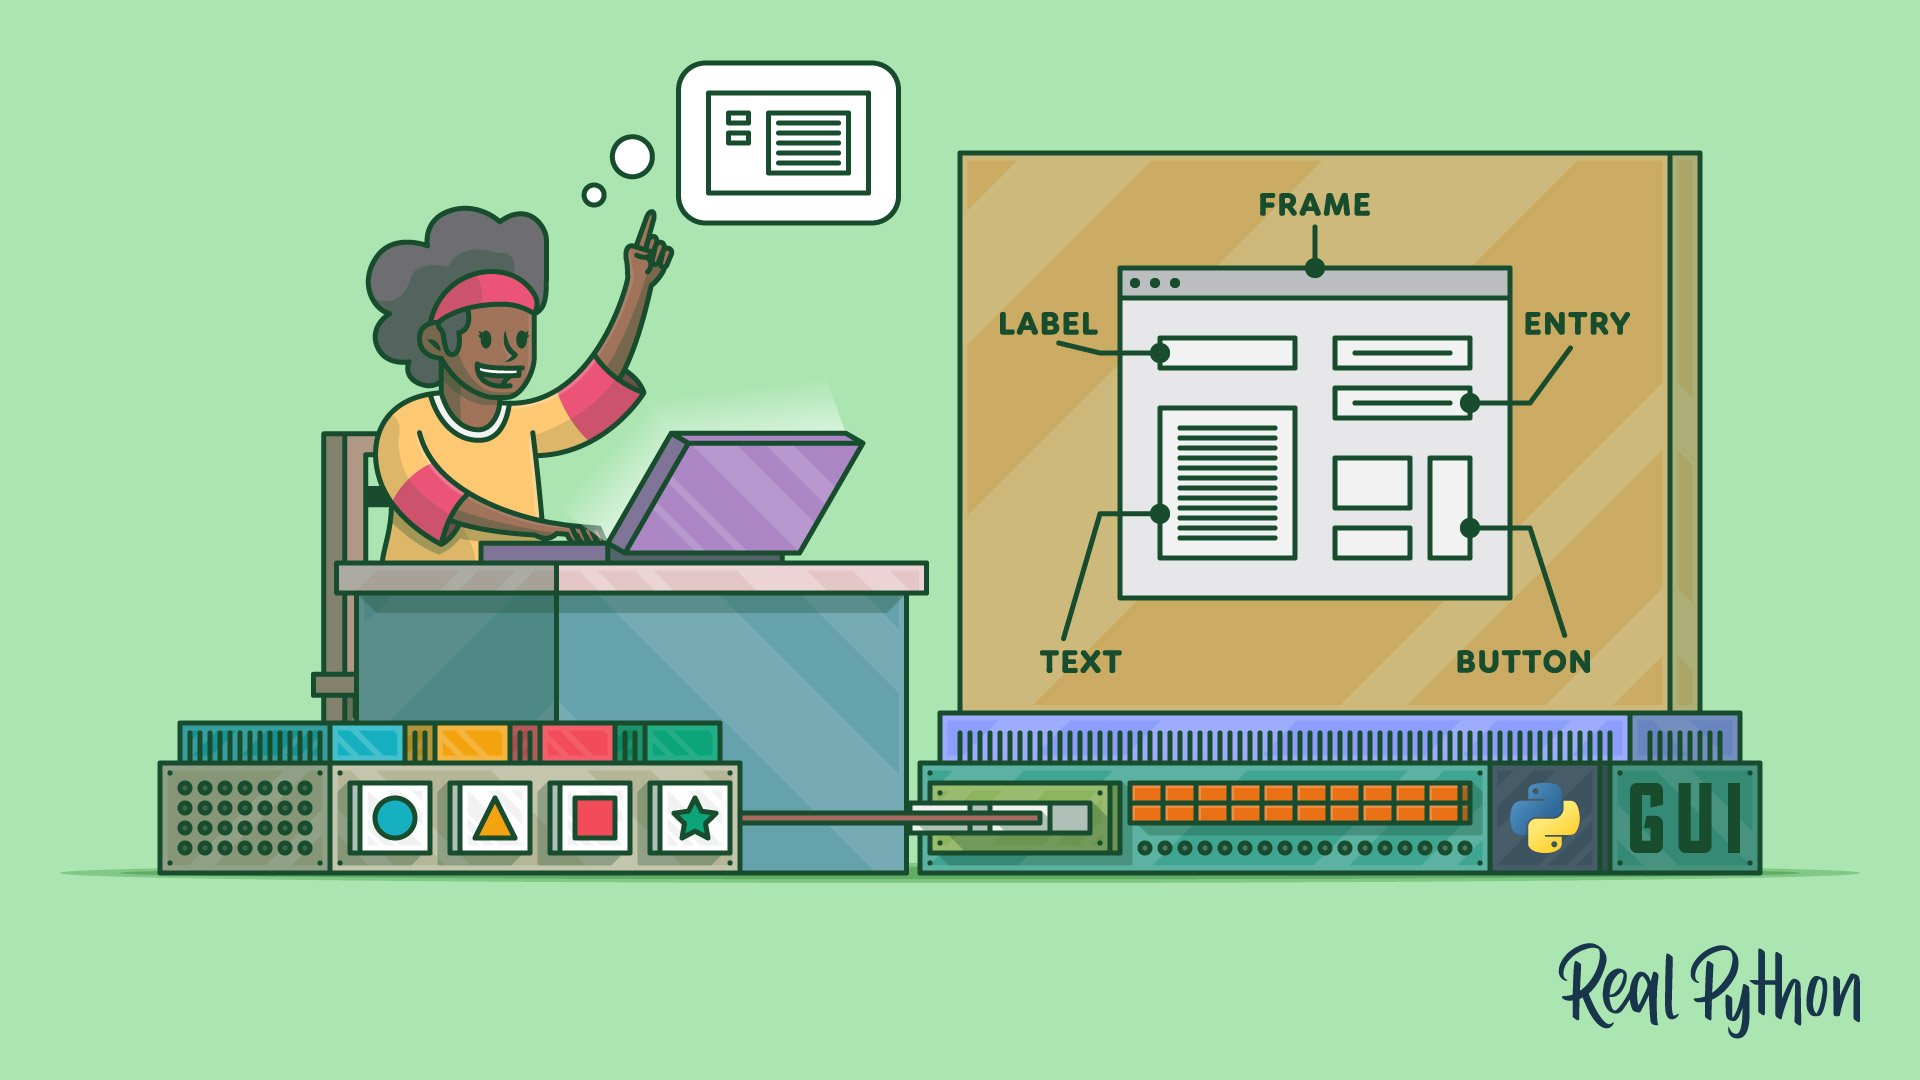
\includegraphics[width=13cm]{images/Tkinter.png}
    \caption{Tkinter}
    \label{Tkinter}
\end{figure}
\subsubsection{OS}
Le module OS de Python fournit des fonctions d'interaction avec le système d'exploitation. Le système d'exploitation relève des modules utilitaires standard de Python. Ce module offre un moyen portable d'utiliser les fonctionnalités dépendant du système d'exploitation. Les modules "os" et "os.path" incluent de nombreuses fonctions pour interagir avec le système de fichiers.\\
\subsubsection{Time}
Le module Time fournit différentes fonctions liées au temps.On a utilisé ce module pour la fonction time.sleep(), cette fonction permet au programme d'obtenir un retard de temps jusqu'à le fichier Dessin.asy s'exécute en donnant l'image Dessin.png a afficher sur dernier interface du programme. 
\newpage
\subsubsection{PIL}
Python Imaging Library (ou PIL) est une bibliothèque de traitement d'images pour le langage de programmation Python. Elle permet d'ouvrir, de manipuler, et de sauvegarder différents formats de fichiers graphiques.\\
La bibliothèque supporte plusieurs formats de fichier, parmi lesquels PNG, JPEG, GIF, TIFF, et BMP.\\
On a utilisé cette bibliothèque pour le traitement et l'affichage des images sur notre application EasyGio ,l'affichage du logo sur les différents pages d'EasyGio et l'affichage du résultat à la fin d'exécution du programme Dessin sous PNG.
\begin{figure}[!h]
    \centering
    
\includegraphics[width=10cm]{images/pillow-logo-248x250.png}
    \caption{Pillow}
    \label{fig:Pillow}
\end{figure}
\chapter{Présentation de l'application}
\section{Interface d'accueil}
\begin{figure}[!h]
    \centering
    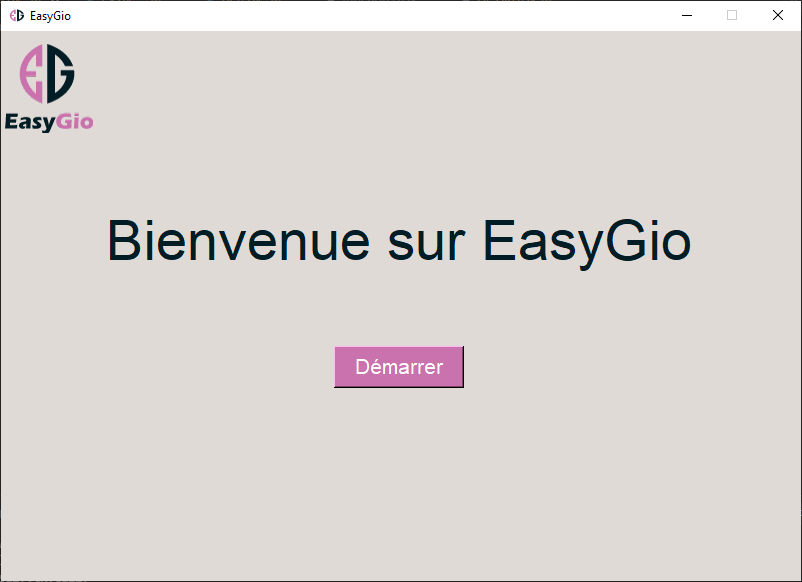
\includegraphics[width=15cm]{images/Interface1.PNG}
    \caption{Interface d'accueil}
    \label{fig:Interface d'accueil}
\end{figure}
Cette interface représente la page d'accueil sur laquelle on peut démarrer notre session en appuyant sur la bouton Démarrer.
\newpage
\section{Interface de choix de section}
\begin{figure}[!h]
    \centering
    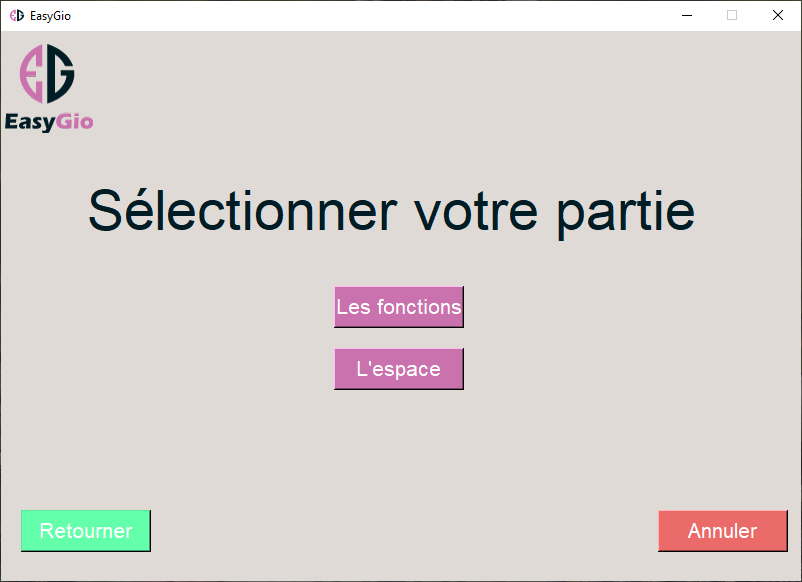
\includegraphics[width=12cm]{images/Interface2.PNG}
    \caption{Interface de choix de section}
    \label{fig:Interface de choix de section}
\end{figure}
Depuis cette interface on peut choisir la partie ou la section voulu.\\
Si on choisit la partie des fonctions on va être rédiger vers une nouvelle page pour choisir le type du fonction Définit ou In-Définit.\\
Et si on choisi la partie de Géométrie dans l'espace on va être rédiger vers nouvelle page pour choisir la partie souhaiter Un sphère, un cube ou la partie des vecteurs.
\section{Interfaces de choix des sous parties}
\begin{figure}[!h]
    \centering
    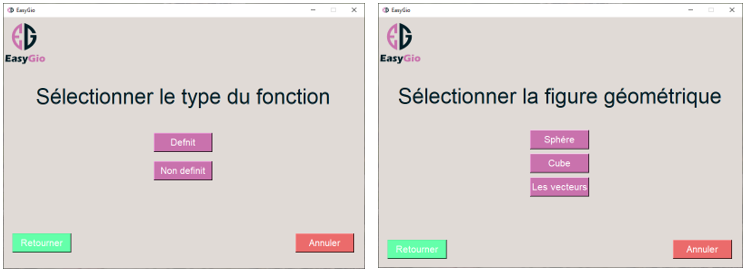
\includegraphics[width=15cm]{images/TypesCaptures.PNG}
    \caption{Interfaces de choix des sous parties}
    \label{fig:Interfaces de choix des sous parties}
\end{figure}
Depuis ces interfaces on peut choisir la sous partie des fonctions et d'espace géométrique.\\
Chaque bouton nous dirige vers une nouvelle page pour saisi les paramètres requit pour chaque diffèrent type.
\newpage
\section{Interfaces des insertion des paramètres}
\subsection{Interfaces des fonctions}
\begin{figure}[!h]
    \centering
    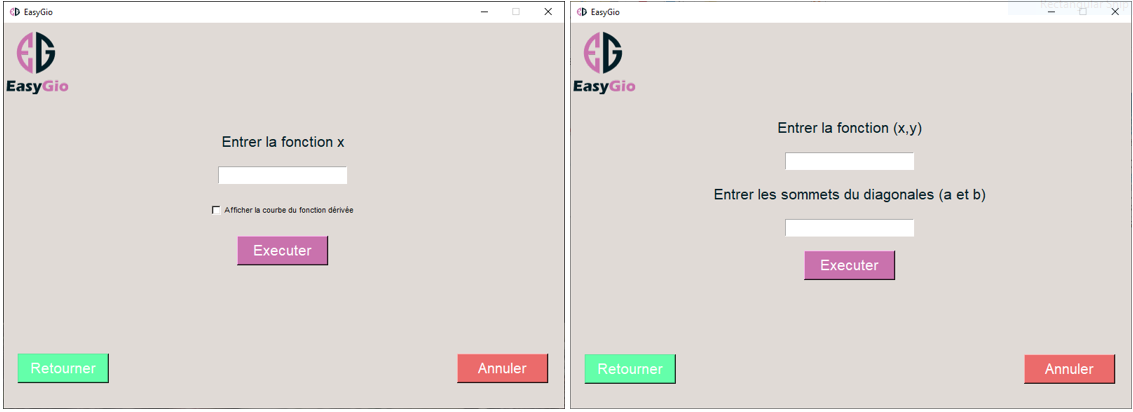
\includegraphics[width=14cm]{images/InputesInter.PNG}
    \caption{Interfaces d'insertion des paramètres des fonctions}
    \label{fig:Interfaces d'insertion des paramètres des fonctions}
\end{figure}
Depuis ces deux interfaces l'utilisateur peut saisir les paramètres des fonction.\\
L'interface à gauche est celle du fonction définit sur la quelle le client doit insérer une fonction d'un seul variable $x$. Et après en cliquant sur la bouton Exécuter le client va être rédiger sur la dernier interface du programme pour l'affichage de la figure sous forme image.\\
L'interface à droit est celle du fonctions Indéfini et sur la quelle l'utilisateur doit saisir une fonction de deux variable $x$ et $y$ et les sommets de la courbe.Et après en cliquant sur la bouton Exécuter le client va être rédiger sur la dernier interface du programme pour l'affichage de la figure sous forme image.\\
\begin{figure}[!h]
    \centering
    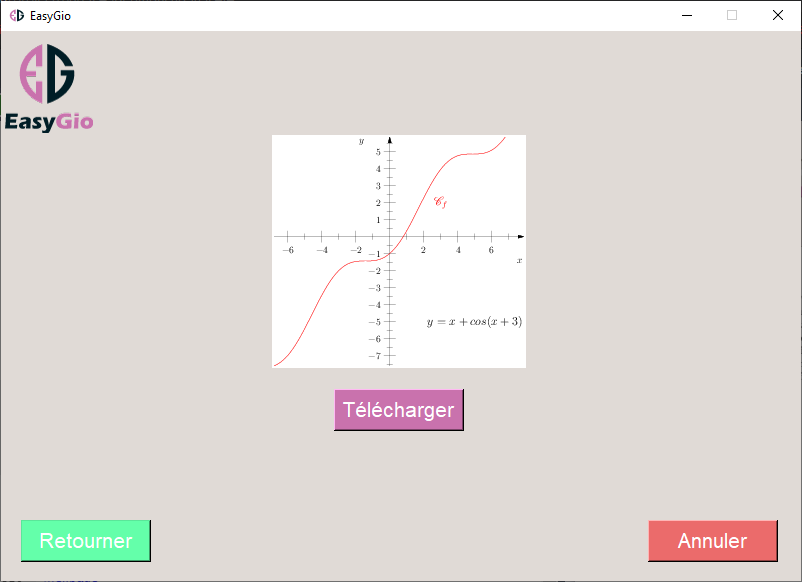
\includegraphics[width=14cm]{images/Fonction.PNG}
    \caption{Exécution d'une fonction (Courbe)}
    \label{fig:Exécution d'une fonction (Courbe)}
\end{figure}
\newpage
\subsection{Interfaces de Sphère et de Cube}
\begin{figure}[!h]
    \centering
    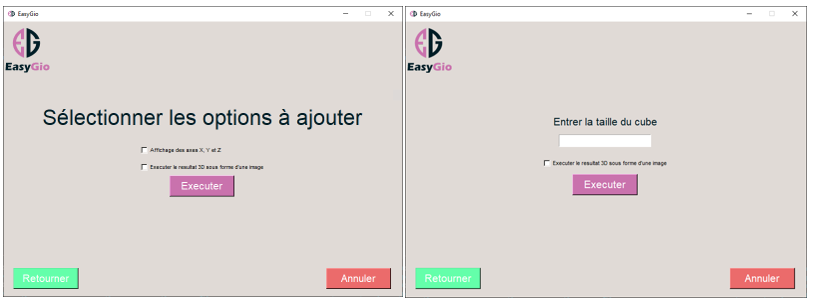
\includegraphics[width=15cm]{images/SpCube.PNG}
    \caption{Interfaces de Sphère et de Cube}
    \label{fig:Interfaces de Sphère et de Cube}
\end{figure}
L'interface à gauche est l'interface pour l'exécution de la figure sphère et sur la quel l'utilisateur a plusieurs choix et options à ajouter, le premier est pour l'affichage des axes X,Y et Z pour le repérage dans le plan et dans l'espace.Le deuxième choix et l'option d'obtenir le résultats final sous forme d'une image PNG à la fin d'exécution du programme. L'utilisateur peut choisir les deux choix à la fois ou un seul choix ou exécuter le programme sans aucun choix.\\
L'interface à droite est celle du Cube où l'utilisateur doit saisir d'abord la taille du cube et qui doit être un nombre entier et supérieur à 0 sinon le système va afficher un erreur.\\
\begin{figure}[!h]
    \centering
    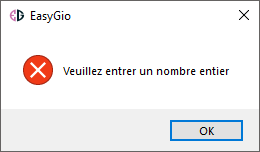
\includegraphics{images/NbError.PNG}
    \caption{Erreur de nombre non entier}
    \label{fig:Erreur de nombre non entier}
\end{figure}
\newpage
La deuxième bouton et le choix d'obtenir le résultat sous forme d'une image PNG à la fin d'exécution du programme ou non. Si l'utilisateur a cocher cette bouton le système va afficher l'exécution du programme sous 3D et après que le client va choisi la positions 3D sur la quelle va obtenir la photo du cube et en cliquant sur la touche 'Q' sur le clavier il va être rédiger sur la page résultat où le système va afficher le résultat sous image PNG.\\
\begin{figure}[!h]
    \centering
    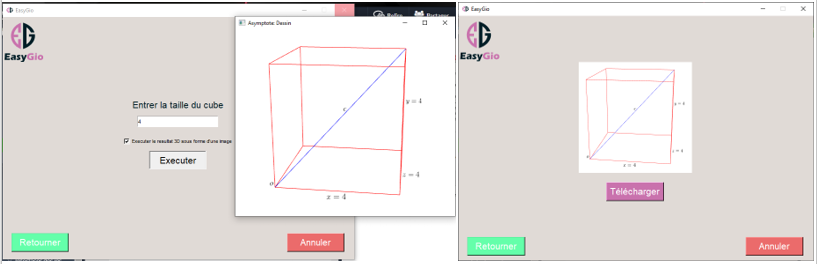
\includegraphics[width=15cm]{images/CubeT.PNG}
    \caption{Exécution d'une figure 3D (cube)}
    \label{fig:Exécution d'un figure 3D (cube)}
\end{figure}
\subsection{Interface de choix des figures pour les vecteurs}
\begin{figure}[!h]
    \centering
    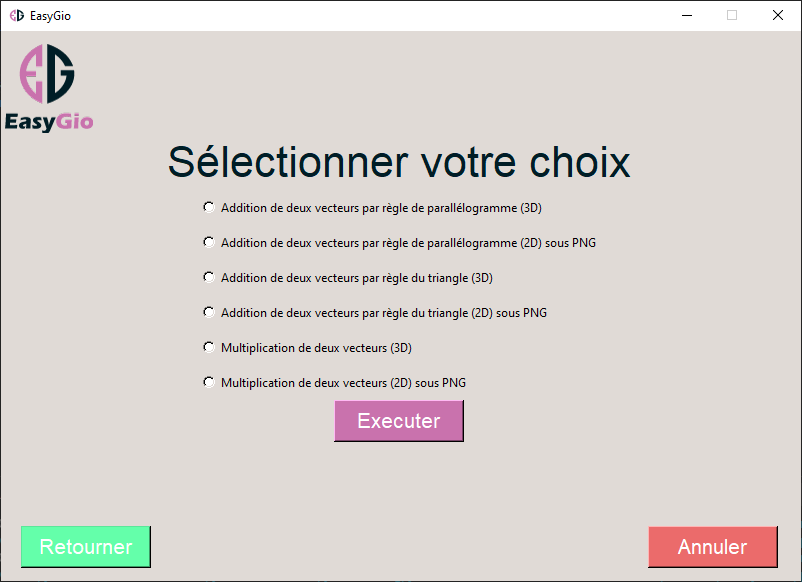
\includegraphics[width=12cm]{images/Vecteur.PNG}
    \caption{Interface de choix des figures pour les vecteurs}
    \label{fig:Interface de choix des figures pour les vecteurs}
\end{figure}
Sur cette interface l'utilisateur peut choisit l'exécution d'une seule figure soit en 3D ou 2D par la quel il va être rédiger sur l'interface du résultat pour l'affichage de l'image PNG:
\begin{itemize}
    \item Addition de deux vecteurs par règle de parallélogramme.
    \item Addition de deux vecteurs par règle du triangle.
    \item Multiplication de deux vecteurs.
\end{itemize}
\subsection{L'interface d'affichage de résultat par Image}
Sur cette dernier interface d'EasyGio il y'a l'affichage de la figure et l'utilisateur peut télécharger sa figure sous forme PNG en cliquant sur la bouton Télécharger avec la quel une fenêtre va être afficher où il peut choisir la position où le fichier Dessin.png va être télécharger.\\
\begin{figure}[!h]
    \centering
    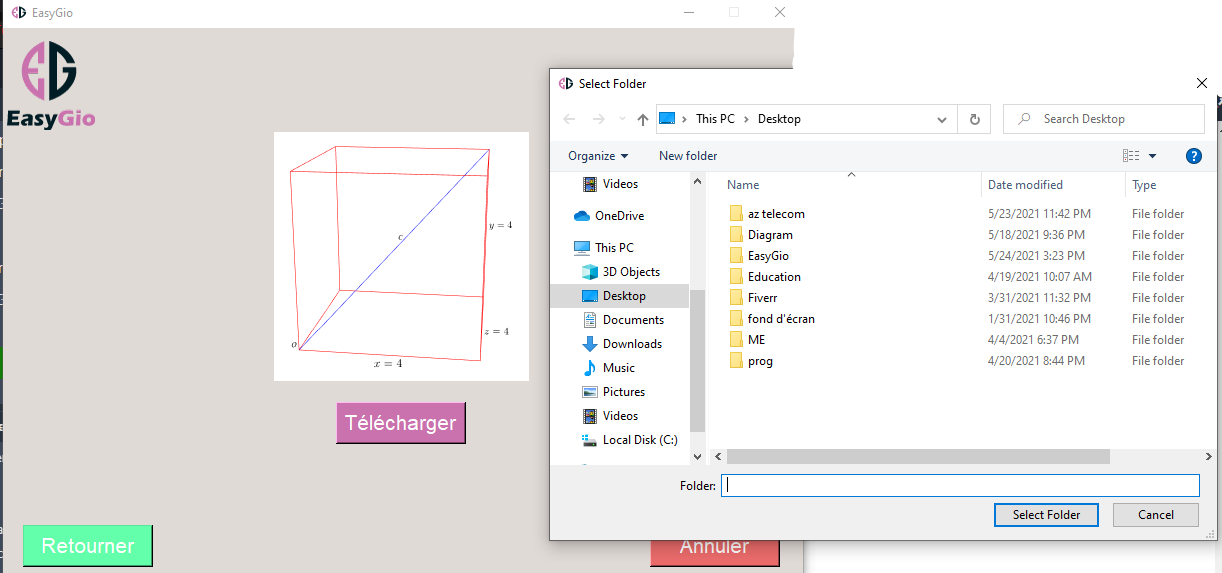
\includegraphics[width=14cm]{images/CubeP.PNG}
    \caption{Choix d'emplacement de téléchargement du fichier}
    \label{fig:Choix d'emplacement de téléchargement du fichier}
\end{figure}\\
Et si le système à rencontrer un problème pour le téléchargement du fichier il va afficher un erreur de téléchargement.\\
Si non il va afficher une notification que le fichier a bien été télécharger.\\
\begin{figure}[!h]
    \centering
    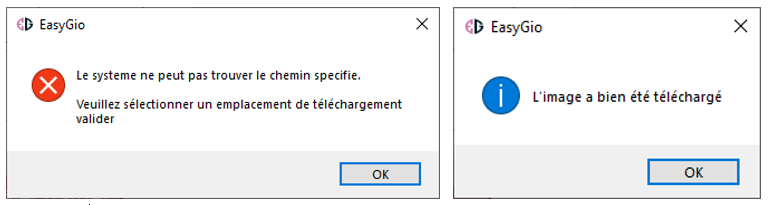
\includegraphics[width=14cm]{images/nots.PNG}
    \caption{EasyGio Info et Erreur fenêtres}
    \label{fig:EasyGio Info et Erreur fenêtres}
\end{figure}
\chapter*{Webographie}
\begin{enumerate}
    \item Google. Le forum officiel d'asymptote pour les documentations\\
    URL: \link{https://asymptote.sourceforge.io}
    \item Google. Un site pour les documents PDF pour comprendre l'asymptote et la bibliotheque Tkinter de python\\
    URL: \link{https://fr.scribd.com}
    \item Wikipedia. Asymptote language\\
    URL: \link{https://en.wikipedia.org/wiki/Asymptote_(vector_graphics_language)}
    \item Google. Démarrage rapide du langage asymptote\\
    URL: \link{https://www.cgmaths.fr/cgFiles/Dem_Rapide.pdf}
    \item Asymptote. A modern successor to the METAPOST vector graphics language\\
    URL: \link{https://www.researchgate.net/publication/242776997_Asymptote_The_Vector_Graphics_Language}
    \item Asymptote. (Vector Graphics Language)\\
    URL: \link{https://artofproblemsolving.com/}
    \item Links to many external resources, including an excellent user-written Asymptote tutorial.\\
    URL : \link{https://asymptote.sourceforge.io/links.html}
    \item A quick reference card for Asymptote.\\
    URL : \link{https://asymptote.sourceforge.io/asyRefCard.pdf}
    \item Google. Le forum officiel de python pour la documentation de la bibliothèque Tkinter\\
    URL: \link{https://docs.python.org/3/library/tkinter.html}
    \item Python Doctor. Interface graphique Tkinter python\\
    URL: \link{https://python.doctor/page-tkinter-interface-graphique-python-tutoriel}
    \item Tutorialspoint. Python guide pour l'interface graphique et la bibliothèque Tkinter \\
    URL: \link{https://www.tutorialspoint.com/python/python_gui_programming.htm}
    \item Realpython. The perfect guid for Tkinter in python\\
    URL: \link{https://realpython.com/python-gui-tkinter/}
    \item Keepscool. Un site web pour les cours du maths au lycée pour avoir les principaux propriétés.\\ 
    URL : \link{http://keepschool.com/fiches-de-cours/lycee/math/vecteurs.html}
    \item Alloschool. AlloSchool est un site de support pédagogique il propose un suivi chronologique par chapitre, comprenant des cours, des exercices corrigés et des examens.\\
    URL : \link{https://www.alloschool.com/}
    
\end{enumerate}
\addcontentsline{toc}{chapter}{Webographie} 
\chapter*{Conclusion Générale et Perspectives}
Étape indispensable lors des cours traditionnels de mathématiques, la géométrie a, de tout temps, souffert d'une réputation de matière difficile ! Des droits parallèles que l'on n'arrive pas à tracer, en passant par une intersection difficile à déterminer, ou des cercles peu assurés, la géométrie est parfois repoussée par les élèves.\\
Pourtant, la géométrie est particulièrement utile dans la vie de tous les jours et permet d'accéder à des carrières prestigieuses comme ingénieur ou chercheur en mathématiques. Autant de professions qui, si elles ne semblent pas être directement liées au quadrilatère et à la demi-droite, le sont bien plus qu'on ne le pense !\\
De plus, la géométrie subit une réputation de branche assez fermée, de domaine dédiée aux matheux et aux matheuses. Contrairement aux apparences, cette branche des maths est accessibles à tous les niveaux et peut même s'avérer être ludique, faisant travailler à la fois sa logique et sa réflexion. Un peu comme les jeux des enfants quoi !\\
\par Les solutions de notre application EasyGio sont des outils indispensables pour répondre à ces exigences. En effet, EasyGio vous permet de construire des multiple figures rapidement et en simple clics. l'application et facilement accessible . Vous pouvait aussi construire des figures 3D et les exporter sous des images PNG avec toute rapidité.\\
\par Malgré les difficultés rencontrées durant ce projet et en particulier le fait de traiter un sujet d’actualité avec peu de documentation, nous sommes parvenues à nous familiariser avec ces nouvelles technologies liées au Asymptote.\\
Et crée une application qui va très faciliter l'illustration des notions de géométrie et surtout dans l'espace à travers notre système des figures 3D en utilisant le langage graphique vectoriel Asymptote pour les enseignants et ces élevés.\\ 
\addcontentsline{toc}{chapter}{Conclusion Générale et Perspectives}
\end{document}